
\documentclass[british,10pt,a4paper]{article}
\usepackage[british]{babel}
\usepackage[margin=1in, bottom=0.75in, top=0.75in, footskip=0.25in]{geometry}
\usepackage[titletoc]{appendix}
\usepackage{fancyhdr}
\usepackage{mathtools}
\usepackage[numbers]{natbib}
\usepackage{filecontents}
\usepackage{pgfplots, pgfplotstable}
    \pgfplotsset{%
    	% every tick label/.append style={scale=1.5},
        compat=newest,%
        /pgf/number format/use comma,%
        /pgf/number format/1000 sep={\,},%
        /pgf/number format/min exponent for 1000 sep=4}
\usepgfplotslibrary{statistics}
\usepackage{hyperref}
\usepackage{booktabs}
\usepackage{wrapfig}
\usepackage{listings}
\usepackage{color}
\usepackage{graphicx}
\usepackage{siunitx}
\usepackage[parfill]{parskip}
\usepackage{tikz}
\usepackage{float}
\usepackage[justification=centering]{caption}
\pgfplotsset{compat=newest} % Allows to place the legend below plot
\usepgfplotslibrary{units} % Allows to enter the units nicely

\graphicspath{ {images/} }

\setcounter{secnumdepth}{2}
\setcounter{tocdepth}{2}
\renewcommand{\arraystretch}{1.2}
\renewcommand\thesection{\arabic{section}}
\renewcommand\thesubsection{\roman{subsection}.}
\renewcommand\thesubsubsection{}
\newcommand*{\Appendixautorefname}{appendix}
\pagestyle{fancy}
\fancyhf{}
\renewcommand{\headrulewidth}{0pt}
\lfoot{Exam no: Y0076159}
\cfoot{\thepage}
\lstset{
  columns=fixed,
  breaklines=true,
  basicstyle=\ttfamily\footnotesize
  }

\usepackage[nottoc]{tocbibind}
\usepackage{csvsimple}

\begin{document}
\title{EVCO Open Assessment}
\author{Exam no: Y0076159}
\date{\today}
\maketitle
\clearpage
\tableofcontents
\clearpage
\listoffigures
\listoftables
\clearpage


\section{Introduction \& Problem Definition}

\begin{minipage}{0.7\textwidth}
The game of Snake was first invented in 1976, as an arcade game named 'Blockade', and later as a computer game named 'Worms' for the TRS-80 microcomputer in 1978 \cite{Goggin2010-ao}; it gained a huge traction on mobile phones following Nokia engineer Taneli Armanto's implementation of the game for the Nokia N6110, released in 2002 \cite{Goggin2010-ao}. The game, in which a single player controls a 'snake' composed of a dot, square or object, is named after the way in which the body of the dot, square or object trails behind the dot controlled by the player. The player can turn the snake's head to change it's direction of travel, whilst the forward movement is uniform relative to time (the player has no control over the speed at which the snake moves). The player aims to win the game by collecting food places on the screen, with every item of food eaten causing the snake's tail to grow. As the player eats more food, the tail grows longer, and it becomes more difficult to navigate the plane without colliding with a surrounding wall, or the player's tail: these form the 2 losing conditions, whilst a player who successfully grows his snake to cover the entire plane has beaten the game.  \newline

Our version of the game is restricted to a 12x12 grid (144 spaces), surrounded by walls, with a single piece of food present on the board at any given time. The snakes starts with an initial length of 11, and is placed facing east with the head at coordinates [11, 4]. Furthermore, the snake can go in any one of 4 absolute directions (up, down, left, right), and always advances by 1 square at a time along either the X or Y axis of the board. As the snake is initialised with a body of size 11, the maximal score obtainable is $144-11=133$), at which point food cannot be placed on a tile not occupied by the snake's body. 
\end{minipage}
\begin{minipage}{0.02\textwidth}
\end{minipage}
\begin{minipage}{0.28\textwidth}
	\begin{figure}[H]
	\centering
		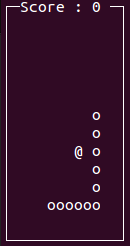
\includegraphics[width=3cm,keepaspectratio]{images/snake.png}
		\caption{A game of snake as simulated in our environment.}
		\label{fig:snake}
	\end{figure}
\end{minipage}

Within the context of this project, we will be aiming to produce an evolutionary algorithm (i.e: an algorithm capable of producing a game-winning A.I. from a set of logical connectives and in-game actions) which can beat the game. That is, we will aim to maximise the number of pieces of food eaten in a run of the game. Key challenges will likely be:
\begin{itemize}
	\item To ensure the snake does not collide into it's own tail or the surrounding walls.
	\item To ensure the snake successfully eats the next piece of food without timing out.
	\item To ensure the algorithm can be run relatively quickly, so it can be evaluated over a large number of runs for statistical analysis.
\end{itemize}

\section{Literature review}
\subsection{Genetic algorithms}
Evolutionary computing is a form of algorithms which seek to find a solution to a problem through a process similar to biological evolution. \cite{Ashlock_undated-vx} The general concept involves initialising a set of candidate solutions, and iteratively updating them to obtain a 'fitter' solution. This is effectively implemented by assessing each candidate using a fitness function, before selecting a a subset of solutions which will be allowed to be bred into child solutions, mutated, and inserted into the next generation's population. This causes the overall fitness of the population to grow over the cycle of evolution, creating a candidate solution which will be closer to the global optimum. Algorithms which implement this evolutionary cycle are known as evolutionary algorithms. The field of evolutionary algorithms (EA) is sub-divided into a series of genetic representations and implementation systems. We will first discuss each of these, highlighting key papers and applications of each to our current situation.\newline

\subsubsection{Genetic algorithm}
A genetic algorithm (GA's) traditionally represent the genotype of a candidate using a binary string, although other representations are possible \cite{Whitley1994-tx}. It is extremely effective at tuning parameters of a model, as demonstrated by \citet{Wloch2004-vo} who used a GA to optimise the parameters of a simulated Formula One car, allowing it to minimise it's lap time. GA's have been implemented for use in the snake game by \citet{Yeh2016-ts}; the algorithm functioned by adjusting the rating functions of 4 operations, each of which decided the snake's next move based on either minimising the number of turns, the free space surrounding the head, or the presence of food near the snake's head. This enabled the snake to evolve a variety of solutions formed of varying frequencies of each function, resulting in a snake capable of beating the game (collecting the maximal number of food possible, where the snake's body fills the entire plane). As the snake's behaviour is not analysed by any means other than it's score in the game, it is difficult to know whether the solution reflected an EA's ability to create novel solutions to the problem. Due to this (and the restrictions on hard-coding solutions to this assessment), an approach using genetic programming was considered, as seen in \autoref{subsec:gp}.

\subsubsection{Genetic programming}
\label{subsec:gp}
Genetic programming (GP) utilises a tree structure to define the genotype of a candidate solution \cite{Cramer_undated-bj}. Nodes in the tree represent certain operators, with leaf nodes representing operands. This allows a decision tree to be evolved, which can rely on conditionally verifying various functions, and applying a move depending on the values of these functions; an example of this is analysed in \autoref{subsec:gp_snake}. Other examples of applications of GPs to games can be found in \citet{Hauptman2005-zg}, who evolved a chess playing agent using a GP. It has also been used in other video games, such as a tower defence game \cite{Leong2013-pu}, space invaders, froggers and missile command \cite{Jia2015-jk}. Within the context of defining a program, GP produce invalid states less frequently than genetic algorithms, as they can be strongly typed (such as in \cite{Jia2015-jk} to ensure that the syntax of the defined operations conforms to an executable standard \cite{Chen2012-ei}. As such, it provides an easily analysable solution to the creation of a snake A.I, as the output of a function is a readily human-readable output. It's additional efficiency in evolving further maximises it's capabilities towards our problem.

\subsubsection{Grammatical Evolution}
Grammatical evolution (GE) presents the next development in EA's; as with genetic programming, it aims to produce a section of code which can define a function, solving the problem at hand. As detailed by \citet{ryan:1998:geepal}, it aims to avoid the requirements of closure imposed on solutions in genetic programming, which are the main causes of bloating and limitations in crossovers. This is circumvented by the use of a user-specific grammar in Backus-Naur form, restricting the search space to only valid individuals. In contrast to a GP, it splits a genotype and phenotype; that is, the objects operated on by the search algorithm differ from those evaluted by the fitness function. This occurs as the grammar is converted into a program through the use of codons, which index the child element to select for each element in a BNF.  As such, GE's provide an escape from the problems suffered by GP's, without adding any significant complexity: this is reflected by a significant improvement in performance when compared to GP's, as demonstrated by \citet{Michael_ONeill1999-zi}. In this paper, GP's and GE's were implemented to solve the Santa Fe ant trail issue, demonstrating a greatly improved fitness for GE's when evolved over the same number of generations as GP's; this is visible in \autoref{fig:gp_vs_ge}. It is therefore apparent that a GE would be more appropriate than a GP to solve the Snake game, but as it is not natively available in the DEAP \cite{deap}, implementing it would go beyond the scope of this project; therefore, a GP will be used.


\begin{figure}
\centering
	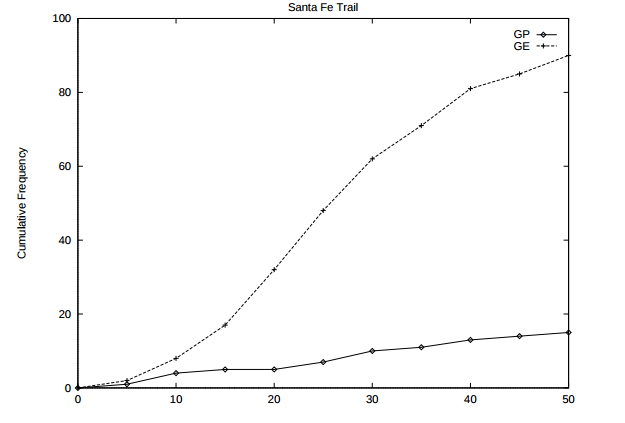
\includegraphics[width=12cm,keepaspectratio]{images/gp_vs_ge.png}
	\caption{GE in comparison to GP, Source: \cite{Michael_ONeill1999-zi}}
	\label{fig:gp_vs_ge}
\end{figure}

\subsubsection{Neuro-evolution}
Neuro-evolution presents the third viable algorithm for the snake game. In this scheme, a neural network's topology and weights are evolved to develop a network which can sense various parameters from it's environment, and output an optimal action back into the game. This was well demonstrated by \citet{Hausknecht2014-uc}, who evolved a single network capable of beating human high scores in a variety of Atari 2600 games. It has also been used to play simple board games, such as Tic-Tac-Toe \cite{Fogel1993-qp}, or GO \cite{Richards1998-si}. As such neuro-evolution is an extremely potent methodology, and further work in it's implementation for the snake game is worthwhile, but it's unavailability in DEAP restricts it's usage for this project. Furthermore, we could hypothesise that a neuro-evolution approach to a simple problem such as the one at hand (relative to playing 61 different games with the same network) may result in a solution which is difficult to analyse, and potentially excessively large in comparison to a GP/GE approach.

\subsection{Co-evolution}
Finally, the last applicable evolutionary technology considered for this application is co-evolution (differential evolution, gene expression programming and evolution strategies were also considered but found to be no more powerful than a GE or GP algorithm within the context of this problem). Co-evolution allows a second population to be evolved in parallel to the first, such that the fitness of an individual in one's population is evaluated using individuals from the other population. This can be combined with any of the previously discussed techniques by running a pair of the algorithms in tandem; however, as we will later detail, it is possible to develop a solution to the snake game which is independent from the size of the map, or the placement of food. As such, there is no competitive development which could be obtained from evolving a map, and therefore co-evolution would not be beneficial to this experiment.


\subsection{Applications of artificial intelligence to Snake}
Some research has also been undertaken to develop intelligent agents for the snake game: \citet{Bowei_Ma_undated-tl} has described an approach to reinforcement learning using Q-learning and SARSA through neural networks, but do not provide any applicable innovation to a GP-based implementation as they use a simple score-based fitness function and a completely different algorithm. \citet{Christopher_Lockhart2010-em} applied back-propagation based learning on neural networks to the game of snake, and implements an improved fitness function which rewards the snake for every unit of time played in the game. \citet{Ehlis2000-sz}'s work (analysed in \autoref{subsec:gp_snake}) is most likely the most applicable research from which to develop our algorithm.

\subsection{Genetic programming for snake}
\label{subsec:gp_snake}
\citet{Ehlis2000-sz} has provided the only comprehensive article specific to the applications of genetic algorithms to Snake. The definitions of the problem diverge from our assessment in a few non-essential ways: snake movements can be inherently defined relative to the snake's current direction (i.e: a turn\_right and turn\_left terminal is defined), and the playing field of the game is a larger rectangle than the 12\*12 field. In all other respects, \citeauthor{Ehlis2000-sz} provides
an overview of a method which functions on the same game as our case. Given this, we will first analyse this approach to the problem, and aim to build an improvement both in terms of computational performance and quality of the solution. \newline

A generic set of terminals allowing the snake to navigate the world is defined: Forward, Left and Right. The latter two allow the snake to make a change of direction relative to it's current heading, whilst the first argument does not affect the heading. The relative movement provided by the two turn operators does allow for a simpler evolution, as implementing an equivalent relative turn using absolute directions requires a significant number of operators, as we will later discuss \autoref{subsec:design_terminals}. \newline

Non terminals can be categorised as either food sensing (ifFoodAhead, ifFoodUp, ifFoodRight) or danger sensing (ifDangerAhead, ifDangerRight, ifDangerLeft, ifDangerTwoAhead). The use of absolute food sensing (ifFoodUp, ifFoodRight) does however require the addition of 4 sensing methods to orient the snake, allowing it to undertake the correct action given the context. This introduces some complexity into the set of operators, potentially limiting the efficiency of the algorithm.\newline

These sets of operators therefore define a generally greedy behaviour: the snake may be progressing towards the food, either at the root of the decision tree or further down once a given situation occurs (such as the 'wall-slitherer' describes in \cite{Ehlis2000-sz}). This evokes a classical approach to the game, similar to what we could expect from the average player\'s strategy. However, given that the last move of a game-winning situation would involve fully covering the map, a greedy approach would need to be very attentive to surrounding dangers to correctly navigate a path to the wall. As such, the difficulty a greedier snake may have in adapting to every potential situation may be the cause for why the algorithm may not produce optimal solutions: an example situation is stated by \citeauthor{Ehlis2000-sz}. This issue forms a basis for the design as later explained. \newline

Some novel features are implemented in this algorithm: the use of multiple evaluations on every snake at every generation cause a larger cost in computational requirements, but do greatly improve the robustness of the solution to food placement and limit the effects of lucky/unlucky food placement on the performance of a snake. Similarly, the fitness function punishes snakes which do not find any pieces of food, thereby promoting snakes which search for the food. The algorithm also relies on priming the population of individuals, by selecting well-performing pre-produced solutions in the initial breeding pool.

Additional details of the algorithm are however lacking: a large population of 10000 individuals is evolved for 500 generations; the large population is potentially a counterweight to the lack of mutation, as unique genomes are created at the start of the evolution rather than during it; this most likely results in an equivalent effect. with a maximum tree size of 150 nodes to limit bloating. Crossover probability is stated as .10 for leaves, 0.80 for nodes, with a mutation probability of 0, in addition to the use of primed populations from previously unsuccessful runs. Additional details concerning which mutation or crossover functions were used are omitted, and reasonable assumptions of these are discussed in \autoref{subsec:impl} to evaluate the method. The algorithm did however account for the randomisation of food placement, mitigating it by evaluating each individual over multiple runs per generation; this was also considered in our algorithm, as we will later discuss.\newline

The proposed solution results in the creation of a game-winning decision tree (which scores the maximal 211 points). This algorithm was re-implemented to establish a benchmark for our research, revealing a significant requirement in computational time, as discussed in \autoref{subsec:impl}.

\subsection{Implementation, assumptions and results}
\label{subsec:impl}

In order to obtain benchmark fitness values, tree sizes and computational times against which to evaluate our new algorithms, the algorithm developed by \citeauthor{Ehlis2000-sz} was implemented using the Python DEAP \cite{deap} package; the code for this can be found in \autoref{app:approach1}. \newline



The algorithm was run 30 times in order to obtain a reliable statistic of it's performance when provided with the population size and computational resources proposed by \citeauthor{Ehlis2000-sz}.



Given that approximately 30 hours of computational time were required to evaluate this, a subsequent evaluation (using a population of 1000, and 150 generations) was run to obtain results against which we can compare our new algorithms quickly. Some assumptions regarding the type of mutation were made: uniform tree insertion was first considered, but as the crossover was set to probability 0, this would be unable to grow the tree. Therefore, a uniform mutation which inserts a subtree of depth 1-3 was utilised. Crossover was set with a probability of 0.0 as per \citeauthor{Ehlis2000-sz}'s design. Finally, we assumed that the fitness tournament was used to drive the population's average fitness upwards: this was implemented with a size of 2, and that a standard evolution algorithm was used (DEAP's eaSimple).\newline

\begin{wrapfigure}{r}{0.5\textwidth}
 	\vspace{-10pt}
	\begin{center}
	  \resizebox {!} {7cm} {
		\begin{tikzpicture}[font=\LARGE]
		    \begin{axis}[xlabel=Food Eaten, ylabel=Count, ybar,xtick=,width=\textwidth]
		    \addplot+[
		    	hist={
		    		data=x,
		    		bins=14,
		    		data min = 0,
		    		data max = 134
		    	}]
		            file [y index=0]  {data/approach1_1000pop.csv};
		\end{axis}
		\end{tikzpicture}
	}
	  \vspace{-20pt}
		\caption{Histogram of best individuals from \citeauthor{Ehlis2000-sz}'s algorithm, 500 generations, 1000 population}
		\label{fig:approach1}
	  \vspace{-10pt}
	\end{center}
\end{wrapfigure}
When limited to a practical computational time (150 gens at 1000 population), the algorithm performs well, with an average of 97.97 pieces of food eaten, and a smaller standard deviation of 29.79 over 30 runs. This highlights the volatility of the algorithm, as well as the need for a large population or a larger number of generation to obtain an optimal value. One should note that the algorithm only has a 16.6\% success rate in producing optimal (game beating) snakes; this is certainly related to the shortening of the algorithm by 350 generations, and the algorithm may therefore be more 
successful than the results above. This was demonstrated in \cite{Ehlis2000-sz}, who finds that given a primed population it is possible to consistently an average max score of the population close to 200. \newline
\begin{wrapfigure}{r}{0.4\textwidth}
  \vspace{-15pt}
  \begin{center}
	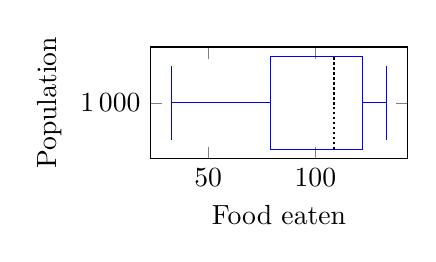
\begin{tikzpicture}
	  \begin{axis}
	    [
	    width=0.4\textwidth,
	    height=3cm,
	    ytick={1},
	    yticklabels={1\,000},
	    ylabel=Population,
	    xlabel=Food eaten
	    ]

	    ] coordinates {};
	    \addplot+[
	    boxplot prepared={
	      median=108.5,
	      upper quartile=122,
	      lower quartile=79,
	      upper whisker=133,
	      lower whisker=33,
	      every median/.style={densely dotted,black, thick},
	    },
	    ] coordinates {};

	  \end{axis}
	\end{tikzpicture}
	  \vspace{-5pt}
		\caption{Results of \citet{Ehlis2000-sz}'s algorithm over 30 runs.}
		\label{fig:box_plot_approach1}
	  \vspace{-10pt}
	  \end{center}
\end{wrapfigure}
This was verified using a second evaluation of the algorithm for 150 generations and 10\, 000 population, as seen in \autoref{fig:box_plot_approach1}. A double tournament was however used to ensure the evaluation could be undertaken given the available resources: this may be the cause of the larger standard deviation of the results, but we can note that as the median of the population is higher in the data with the larger population, we can expect the algorithm to perform. It is therefore possible that our final algorithm would perform better than the results detailed in this report if given a larger population or number of generations; this would have to be verified in the work's extension.\newline 

Nevertheless, we can establish a benchmark against which we can compare future algorithms, keeping in mind the scale of resources provided to the algorithms is limited given available computing power. This can most easily be described as an average best score of 97.97  (std: 29.79), given 150 generations with a population of 1000, with an average tree size of 362.8 nodes. \newline




\section{Testing \& Design methodology}
\label{sec:methodology}
In order to evaluate the effects of operators or fitness functions, each candidate fitness function will be evaluated 30 times, with a consistent configuration: a population of 1000 individuals evolved over 150 generations. These parameters allow us to evaluate the solutions rapidly, but results should be considered with the assumption that a larger population and number of generations would improve the score and consistency of the algorithm, in the same way our restricted implementation of \citet{Ehlis2000-sz}'s algorithm underperforms compared to the extensive experiment performed in that report. We will aim to create an algorithm which requires less computational power, and produces optimal results more consistently with a smaller population and tree size. Fitness functions will be evaluated using the same algorithm (eaSimple), although a later comparison of algorithms will be run. Finally the optimal mutation and crossover probabilities will be found by iterating combinations of them with the most promising algorithm. As the benchmark algorithm discussed in \autoref{subsec:impl} does not produce normally distributed data (as visually verifiable using the graph), a Mann-Whitney U-test will be used to compare the score of subsequent algorithms, as it does not rely on the assumption of normal distributions\cite{Timm2002-lo}.  The two tailed variation of the U-test will be used, to ensure both algorithms can be found to be statistically better than the other. A p value of 0.05 will be used as a level of statistical significance.\newline


\section{Design \& implementation}
\subsection{Evolutionary algorithm}
A genetic programming algorithm was used, as it provided the most flexibility available from the DEAP package in terms of the solution space explored as it utilised a large number of operators, each with a small individual impact over the snake's movement, in comparison to an implementation which utilised a genetic algorithm such as \citet{Yeh2016-ts}.

\subsection{GP Algorithm selection}
Two categories of complete algorithms were considered for this experiment: DEAP's eaSimple, which implements the basic evolutionary algorithm as defined in \citet{Back2000-og}, and the newer lambda algorithms which implement forms of elitism (eaMuCommaLambda and eaMuPlusLambda). DEAP's eaSimple was chosen to increase the consistency of the algorithm, as it does not force elitism in the early generations of the algorithm; this permitted a larger variety of genotypes, thereby maintaining a diverse population of individuals throughout the evolution to maximise the probability of the correct mutations occuring. In contrast to this, we would expect the lambda-based algorithms to converge much more rapidly, although this effect can be managed using the parameters of the algorithm. Given the complexity of finding an additional 5 parameters of a lambda algorithm (mutation rate, crossover rate, number of individuals to select from current generation, number of children to produce at each generation), it would be most effective to implement a meta-genetic algorithm to find near-optimal parameters for a lambda algorithm. Given this data, and an equivalent optimisation of an eaSimple-based algorithm, we could conduct a statistical analysis of the two sets of data, and thereby find an optimal algorithm. However, for the purpose of this research, we will aim to optimise the parameters of an eaSimple and tournament selection so as to best cover the search space offered by both eaSimple and lambda algorithms.

\subsection{Strategy}
As \citet{Ehlis2000-sz} has already demonstrated a game-beating A.I, it was decided to focus on 3 aspects which we could compare to this algorithm:
\begin{itemize}
	\item Equalling or beating the reliability of the algorithm
	\item Reducing the computational time
	\item Reducing the size of the average game-beating solution
\end{itemize}
Building on the work by \citeauthor{Ehlis2000-sz}, we will aim to adapt his design to our requirements whilst improving it. As noted by \citet{Christopher_Lockhart2010-em} in his publication about difference learning in Snake, "the greedy behaviour of [a learning agent] may be the cause of the agent's lack of high scores. Whilst this is disproven by the success rate of \citeauthor{Ehlis2000-sz}'s algorithm, we could argue that given a sufficiently large population, a set of operators can produce any solution which could also be produced by a subset of those operators. We attempted to demonstrate this in \autoref{app:operator_prob}, where we compiled statistics from the best individuals of optimal (game-winning with a score of 133) and non-optimal solutions, across 30 runs with a population of 10 000 and 150 generations. As we can see, there is no noticeable difference between the frequency of operators, thereby demonstrating that not all optimal solutions are greedy, as this would be reflected by a lower percentage of food sensing functions (redundancies in the graphs (such as repeated operators or unrecheable branches) and noise in the data obtained may also have obscured any visible pattern). Nevertheless, we will hypothesise that developing a non-greedy snake may have the following benefits:

\begin{itemize}
	\item A greedy snake which alters it's movement based on the positioning of food is likely to require additional sensing to avoid going causing game-ending situations, such as entering a dead-end to get closer to a piece of food. This would require the handling of many edge cases, which will cause the need for a large solution, which is therefore difficult to evolve. A non-greedy snake, which would aim to find a hamiltonian cycle through the map such that it's tail will never be in it's direct path until it has reached maximal size, could require a significantly smaller function to define it; this should make it easier to evolve, and therefore increase the reliability and speed of the algorithm.
	\item As a non-greedy snake would not sense food, it's fitness is unlikely to be greatly affected by the positioning of food. Therefore, it may not be necessary to evaluate each individual multiple times, which was done to improve the robustness of the solution in \cite{Ehlis2000-sz}.
\end{itemize}
Due to this, it was decided to aim for a non-greedy solution which would not sense for food, but would rather aim to explore the map in a maximal way; this would adequately resolve the prescribed goal of beating the game by obtaining a maximal score, even though it may not be achieved in a minimalistic way.

\subsection{Terminal and Non-terminal set}
\label{subsec:design_terminals}
The most significant difference of environment between our project and previous work involves the added complexity of using only absolute turning: as such, instead of a simple \texttt{turn\_left} and \texttt{turn\_right} function, we implement changeDirectionUp, changeDirectionRight, changeDirectionDown, changeDirectionLeft; these allow the snake's head to progress towards one of 4 directions at the next move. As these directions are difficult to use without any knowledge of the current heading (e.g: turning down when going north would cause the snake to reverse into it's own body), an additional 4 senses are used: \texttt{if\_moving\_up}, \texttt{if\_moving\_down}, \texttt{if\_moving\_left}, and \texttt{if\_moving\_right}. \newline
\begin{wraptable}{r}{0.35\textwidth}
	\centering
	\begin{tabular}{|l|l|}
		\hline
		\textbf{Terminal} & \textbf{Non-terminal} \\ \hline
		go\_straight      & if\_wall\_2\_away     \\ \hline
		go\_up            & if\_wall\_left        \\ \hline
		go\_down          & if\_wall\_right       \\ \hline
		go\_right         & if\_wall\_ahead       \\ \hline
		go\_left         & if\_moving\_up        \\ \hline
		                  & if\_moving\_down      \\ \hline
		                  & if\_moving\_left      \\ \hline
		                  & if\_moving\_right     \\ \hline
	\end{tabular}
	\caption{Operators}
	\label{tab:operators}
\end{wraptable}
As we will aim for a non-greedy solution, food sensing is not implemented in the new algorithm. We will aim to produce a hamiltonian cycle (where every space of the bordered plane is visited only once before returning to the original), as this will avoid having to take the snake's tail into consideration. Therefore, we will implement 4 wall-sensing functions: \texttt{sense\_wall\_ahead, sense\_wall\_left, sense\_wall\_right \& sense\_wall\_2\_away}. The first 3 of these are relative to the snake's orientation, and allow the snake to navigate against a wall, whereas the $4^{th}$ sense allows the snake to avoid completely traversing the map along either the X or Y axis, thereby permitting it to avoid cutting itself off from part of the map which will be made available as it continues to move. This represents a generalisation of two operators proposed by \citet{Christopher_Lockhart2010-em}: danger forward two, and danger right two.\newline


Some additional tests were conducted to determine alternative operators to \texttt{if\_wall\_2\_away}) (set 3): more specific operators (such as \texttt{if\_wall\_2\_ahead} or \texttt{if\_wall\_2\_right}) were evaluated in place of the aforementioned operator, and resulted in a worse performance. This was evaluated over 30 runs with each set of operators, using the fitness function defined in \autoref{subsec:fitness_func}, with a crossover probability of 0.8, a mutation probability of 0.7, a doubleTournament selection of size 5 with a parsimony value of 1.05 and fitnessFirst=True, using DEAP's eaSimple GP algorithm. Other operators included in the evaluation were all 5 terminals, all 4 orientation sensing, and all wall sensing of distance 1 (\texttt{if\_wall\_ahead}, \texttt{if\_wall\_right} and \texttt{if\_wall\_left}). \newline

\begin{table}[ht]
	\centering
	\begin{tabular}{|l|l|l|l|}
	\hline
	 & Set 1 & Set 2 & Set 3 \\ \hline
	Alternative wall sensing operators & \texttt{2\_left}, \texttt{2\_right}, \texttt{2\_ahead} & \texttt{2\_right}, \texttt{2\_ahead} & \texttt{2\_away} \\ \hline
	Avg score & 26.198 & 27.626 & 47.2915 \\ \hline
	STD & 43.874 & 45.570 & 57.791 \\ \hline
	Optimal runs & 1 & 3 & 6 \\ \hline
	Ratio of perfect scores & 0.05 & 0.15 & 0.3 \\ \hline
	\end{tabular}
	\caption{Comparison of operator sets}
	\label{tab:operator_comparison}
\end{table}
\begin{wrapfigure}{r}{0.4\textwidth}
  \vspace{-20pt}
  \begin{center}
	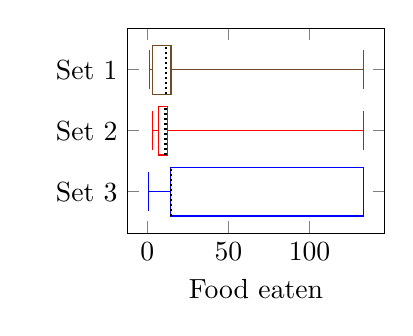
\begin{tikzpicture}
	  \begin{axis}
	    [
	    width=0.4\textwidth,
	    ytick={1,2,3},
	    yticklabels={Set 3, Set 2, Set 1},
	    xlabel=Food eaten
	    ]

	    \addplot+[
	    boxplot prepared={
	      median=14.64,
	      upper quartile=133,
	      lower quartile=14.5,
	      upper whisker=133,
	      lower whisker=0.77,
	      every median/.style={densely dotted,black, thick},
	    },
	    ] coordinates {};
	    \addplot+[
	    boxplot prepared={
	      median=11.12,
	      upper quartile=12.5175,
	      lower quartile=7.0725,
	      upper whisker=133,
	      lower whisker=2.93,
	      every median/.style={densely dotted,black, thick},
	    },
	    ] coordinates {};
	    \addplot+[
	    boxplot prepared={
	      median=11.325,
	      upper quartile=14.5975,
	      lower quartile=3.24,
	      upper whisker=133,
	      lower whisker=1.47,
	      every median/.style={densely dotted,black, thick},
	    },
	    ] coordinates {};
	  \end{axis}
	\end{tikzpicture}
	  \vspace{-5pt}
		\caption{Comparative plots of operator sets described in \autoref{tab:operator_comparison}}
		\label{fig:box_plot_operators}
	  \vspace{-10pt}
	  \end{center}
\end{wrapfigure}
This resulted in \autoref{tab:operator_comparison}: as we can clearly see, the smaller, more generic operator set consisting of the aforementioned operators in addition to if\_wall\_2\_away (which returns true if the snake's head is 2 spaces away from a wall in any direction) results in a consistently better fitness. This is reflected by the difference in averages, and is confirmed to be statistically significant by the Mann-Whitney U-test values: set 3 has a higher median than set 1, with a Z-score=2.489, U=180.5 and p=01278, and set 3 also has a higher median than set 2 with a Z-score=2.682, U=170.5, p=0.00736. The third set is therefore statistically superior to other proposed operator sets, and will be used to evaluate in our algorithm, as detailed in \autoref{tab:operators}. These were not implemented as a strongly typed primitive set, as there were no variations in the types of terminal or non-terminal operators which could cause un-evaluable solutions. Additionally, the conditions were implemented as part of an if\_statement structure as their use in any other part of the tree would result in an invalid individual, unless a strongly typed set was implemented (which would have resulted in an additional overhead).

\subsection{Fitness function}
\label{subsec:fitness_func}
Keeping in line with the aim of a greedy snake, our fitness function does not include the snake's score in the game; this is due to the fact that snakes cannot sense food, and therefore their score will be directly correlated with the distance travelled by the snake (and therefore it's distance travelled, as it moves at a constant speed). In addition, as the snake's score can greatly be influenced by the random placement of food in the starting few generations, removing the scoring of food reduces the skewing of a snake's fitness due to lucky food placing. This further reduces the need to evaluate each snake multiple times, as the snake only reacts relative to constant objects in the plane (4 walls). Finally, to ensure the hamiltonian cycle covers every square of the map, we introduce the notion of a cover to the fitness function, which is equal to the proportion of the map visited by the snake during the run. This ensures that snakes develop a maximal coverage of the map, so that it can grow to a maximal size. \newline

We can therefore define the fitness function as \(fitness= (\% \ of\ map\ covered) + (steps/100)\). \newline
In addition to this, we also implemented a penalty for snakes which enter a non-maximal loop: this is implemented by checking if the snake has timed out (i.e has travelled 196 steps without collecting food). This removes problematic solutions from the early stages of evolution, as these individuals would otherwise score highly due to their long survival; instead, they will now be assigned a fitness of -10, thereby greatly reducing their likelihood of selection, and therefore their effect on the population's genotype.

\subsection{Creation of individuals}
\subsection{Selection, Mutation \& Crossover}
In contrast to \citeauthor{Ehlis2000-sz}'s algorithm, which relied on the insertion of tree structures in the place of individual nodes (using mutUniform)  to grow a solution beyond it's initial size (as crossover probability was set to 0), our genetic algorithm utilises crossover throughout it's evolution. Therefore, it was possible to rely on crossover to grow a tree's size, whilst DEAP's mutNodeReplacement operator, which replaces a primitive from an individual by any other primitive which has the same number of arguments, was used to mutate individuals. This allows nodes within the tree to be replaced with more appropriate nodes, thereby improving their fitness. The basic one point crossover operator was used, without bias for leaf nodes. \newline

As details of the selection algorithm in \cite{Ehlis2000-sz} are sparse, we decided to utilise a double tournament, to ensure that the size of the solutions was minimised given an equal fitness. As such, DEAP's doubleTournament implementation allows the size of individuals to be minimised without greatly hampering the fitness of the population. The parameters for the mutation rate, crossover rate, tournament size and parsimony can be found in \autoref{sec:params}.\newline

\subsection{Parameter selection}
\label{sec:params}

In order to obtain a tuple of parameters (crossover probability, mutation probability, selection tournament size, parsimony), a search across pairs of crossover and mutation probabilites was undertaken. This was implemented using the set of operators defined in \autoref{tab:operators}, using DEAP's eaSimple algorithm Each combination of probabilities (in increments of 10\%) was evaluated 5 times, and it's average was plotted in \autoref{fig:mutpb_cxpb}. Additional runs would have been beneficial to the overal smoothness of the graph, as outlying runs may have a strong impact on the averaged value. Nevertheless, an optimal mutation rate of 0.8 and a crossover rate of 0.7 were chosen as the best parameters. The same search was repeated over tournament size (range from 2 to 7 in integer increments) and parsimony (range from 1 to 2 in 0.05 increments), as seen in the 3d plot \autoref{fig:fitness_parsimony}. This yielded a best parsimony and selection tournament size of (1.05, 6), with an average 116.12 pieces of food eaten. The small parsimony size would certainly have allowed the individuals to maximise fitness rather than size, causing more bloat and slowing the solution, but increasing the number of optimal individuals in the run. The high fitness tournament size is effectively implementing a form of elitism, and we could expect that as we increase the tournament size we would approach the behaviour of the Mu-Comma-Lambda or Mu-Plus-Lambda algorithms (where the fittest n \% of a population are maintained and reproduced to create a proportion of the next generation).\newline

The population size was kept at 150 to allow for a statistical comparison of our algorithm within the timeframe of this project.

We should note that this method suffers from the assumption of independence between the two searches; that is, crossover probability and mutation rates affect the population's fitness independently to the selection tournament's fitness size and parsimony. This approach was selected to maximise the success of the algorithm given the constraints of this project; an alternative approach could be to implement a genetic algorithm which could alter these four parameters, and evolve an optimal parametrisation of our current algorithm. This method is known as a meta-genetic algorithm, and was succesfully used by \citet{Brain2011-pz} to parametrise the crossover rate, mutation rate, tournament selection method and population size of another genetic algorithm. Therefore, the full set of parameters for our genetic algorithm could be determined by a meta-genetic algorithm, given sufficient computational power and time.\newline

\subsection{Creation of individuals}
Individuals were generated using the ramped half and half method proposed by \citet{Koza1992-zm}. This algorithm randomly picks a value within the size range provided, and with .5 probability uses a GROW algorithm to generate a tree, or generates a full tree of that depth. \cite{Luke2001-ix}. While \citet{Luke2001-ix} does not find any benefit of this algorithm towards the final fitness of the algorithm, the ability to avoid specifying an exact depth helps to reduce the dimensionality of the parameters of the algorithm; \citeauthor{Luke2001-ix} does note that having a distribution of initial sizes increases the probability of generating good initial individuals. As such, it was decided to use the ramped half and half generation to produce a diverse set of individuals which we can then evolve into a solution.

\subsection{Bloat control}
Bloat control was implemented using decorators on the crossover and mutation functions, limiting the height of an individual's tree to 7. In addition, the use of a double tournament effected minimal pressure on the population, to avoid greatly hindering the algorithm's ability to find optimal solutions to the game. The combinations of these contributed to creating an algorithm which is quicker to run than previous illustrated \cite{Ehlis2000-sz}; this will be evaluated in \autoref{subsec:results_time}.

\subsection{Code optimisation}
\label{subsec:code_optimisation}
A series of optimisations were undertaken to improve the performance of our algorithms. Firstly, the timeout limit of a snake's run, which causes a snake to 'die' after a certain time has passed since it has last eaten food, was reduced to the size of the board. This allows earlier generations, where looping snakes occur the most, to end before any un-necessary computation occurs. \newline
The body of the snake was re-implemented using python's Deque collection \cite{noauthor_undated-bi}, which is optimised for fast appends and pops on either end of the list-like container. The food positioning algorithm was improved, such that instead of randomly selecting a tile in the plane before checking it would be a valid space for food, the algorithm instead creates a list of free spaces, and randomly selects one from that list. This flattens the response time of the algorithm, which would most likely have been faster at the start of the game, but would require a significant number of queries before randomly finding an available tile. Finally, python's MultiProcessing module was added to the project, which allowed the evaluation of a generation of snakes to occur in parallel over a large number of cores, thereby greatly reducing the computational time required per generation. Multiprocessing was conditionally removed from the code to evaluate it's computational time relative to \citet{Ehlis2000-sz}, and is also un-used when the algorithm is provided with a seed (as this causes the execution to become non-deterministic).

\subsection{Algorithm summary}
Our algorithm can be summarised as follows:
\begin{itemize}
	\item Population: 1000, Generations: 150
	\item Mutation probability: 0.8, Crossover probability: 0.7
	\item Selection process: Double tournament, fitness first with tournament size of 6 and a parsimony of 1.05
	\item Crossover algorithm: cxOnePoint
	\item Mutation algorithm: mutNodeReplacement
	\item Maximum tree depth decorators: max depth of 7 on crossover and mutation.
	\item Creation of individuals: ramped (half and half) in range [2,6]
	\item Operator set: as described in \autoref{tab:operators}.
	\item Fitness function: \% of map covered + (number of steps taken/100), or -10 if the snake has timed out

\end{itemize}

\section{Results and analysis}
\subsection{Executing the algorithm}
\label{subsec:results_score}
\begin{wrapfigure}{r}{0.4\textwidth}
	\centering
	\vspace{-30pt}
		\begin{tikzpicture}
			\begin{axis}[
				grid=major,
				ymin=0,
				xlabel=Pieces of food eaten,
				ylabel=Frequency,
				width=0.4\textwidth,
				height=6cm,
				ybar
				]
				\addplot +[
				red!60,
				fill opacity=0.8,
				hist={
				    bins=15,
				    data min=0,
				    data max=134
				}   
				] table [y index=0] 
				{data/approach4.csv};
				\addplot +[
				blue!60,
				fill opacity=0.5,
				hist={
				    bins=15,
				    data min=0,
				    data max=134
				}   
				] table [y index=0,col sep=comma] 
				{data/approach1_1000pop.csv};
				\legend{New algorithm, \citeauthor{Ehlis2000-sz}}
			\end{axis}
		\end{tikzpicture}
	\vspace{-10pt}
	\caption{Histogram of the best individual in the population}
	\label{fig:approach1_vs_approach4}
	\vspace{-30pt}
\end{wrapfigure}
The Python 2.7.6 code for our new algorithm can be found in \lstinline{new_algo.py}. An optimal run can be obtained by running the following command: 
\lstinline{python new_algo.py --seed 0.507299291138 --max_gen 50}

This will also display the optimal snake in game. Additional parameters can be passed to the algorithm (if no seed is specified):
\begin{itemize}
	\item to run the algorithm multiple times (add arguments \lstinline{--iterations n}), 
	\item to run it for a different number of generations (\lstinline{--num_gen n}), 
	\item to run it using Python's multiprocessing module (\lstinline{--multicore}, note that this results in a non-deterministic execution due to process-specific calls to Python's random module), 
	\item to create a .csv and save the result of the execution (\lstinline{--save_results}).
\end{itemize}

\subsection{Game score maximisation}

\begin{table}[b]
	\centering
	\begin{tabular}{|l|l|l|}
	\hline
	 & Ehlis & New algorithm \\ \hline
	Median & 108.5 & 47.15 \\ \hline
	std & 29.79294447 & 55.98871726 \\ \hline
	Proportion of optimal solutions & 0.167 & 0.34 \\ \hline
	\end{tabular}
	\caption{Average best score (food eaten) over 30 executions}
	\label{tab:algo_score_comparison}
\end{table}
Following the methodology defined in \autoref{sec:methodology}, our new algorithm was evaluated 30 times using the best parameters found in \autoref{sec:params}, and the results of this experiment were compared to our implementation of \citet{Ehlis2000-sz}'s algorithm from \autoref{subsec:gp_snake}. As we can see in \autoref{fig:box_plot_algorithm_perf}, our algorithm performs worse than our benchmark on average. After testing the distribution of both data sets for normality using a Shapiro-Wilk normality test \cite{Shapiro1965-my} (benchmark data is not normally distributed with W=0.9127, p<0.05, nor is our data with W=0.6211, p<0.01), we confirmed the statistical significance between the algorithms using a Mann-Whitney U-test on the sets of best scores from runs of each algorithm (U=247.5, p-value of 0.00174) and the difference in median scores seen in \autoref{tab:algo_score_comparison}. Our algorithm is therefore no better than our benchmark implementation in terms of the average max fitness. However, our new algorithm does produce a larger number of optimal solutions, at a rate of 0.34 vs the previous best of 0.167: this is reflected in \autoref{fig:approach1_vs_approach4}, where our algorithm forms two spikes at the bottom and top of the x axis. \newline

The implementation of our non-greedy strategy through our fitness function and non-greedy operator set has resulted in a binary result: either a full hamiltonian cycle is found, which allows the snake to win the game regardless of the placement of food, or the snake fails to form a complete path and zig-zags the plane without leaving a path for it to travel back through the map. As such, we have demonstrated that a non-greedy solution can be as effective as a greedy approach to solving the Snake game, but may require a larger population or number of generations to achieve a consistent average score.




\begin{wrapfigure}{t}{0.4\textwidth}
  \vspace{-20pt}
  \begin{center}
	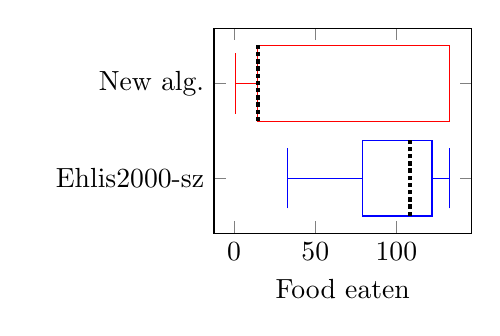
\begin{tikzpicture}
	  \begin{axis}
	    [
	    width=0.4\textwidth,
	    ytick={1,2},
	    yticklabels={\citeauthor{Ehlis2000-sz}, New alg.},
	    xlabel=Food eaten
	    ]
	    \addplot+[
	    boxplot prepared={
	      median=108.5,
	      upper quartile=122,
	      lower quartile=79,
	      upper whisker=133,
	      lower whisker=33,
	      every median/.style={densely dotted,black, ultra thick}
	    },
	    ] coordinates {};

	    \addplot+[
	    boxplot prepared={
	      median=14.64,
	      upper quartile=133,
	      lower quartile=14.5,
	      upper whisker=133,
	      lower whisker=0.77,
	      every median/.style={densely dotted,black, ultra thick}
	    },
	    ] coordinates {};
	  \end{axis}
	\end{tikzpicture}
	  \vspace{-20pt}
		\caption{Comparison of algorithm performance}
		\label{fig:box_plot_algorithm_perf}
	  \vspace{-10pt}
	  \end{center}
\end{wrapfigure}

\subsection{Computational time reduction}
\label{subsec:results_time}
Our second objective involved reducing the computational time required to run the algorithm whilst maintaining a similar level of optimality. Whilst the latter objective was not achieved, our algorithm is significantly faster to execute, as detailed by the box plot in \autoref{fig:box_plot_algorithm_time}. The median values were 824.9 seconds for the benchmark implementation, and 115.8 seconds for our algorithm. As neither data set is normally distributed (benchmark dataset: W=0.648 p<0.01, our dataset: W=0.860, p<0.01, using a Shapiro-Wilk normality test), a Mann-Whitney U test demonstrated that our algorithm is significantly faster with U=5 p<0.0001. Therefore we may conclude that we have produced a significantly quicker algorithm, to the point where we may consider the following: given an equal amount of time, multiple executions (approximately 7) of our algorithm could be performed in the time taken by a single execution of the benchmark. Given the 0.33 percent chance of finding an optimal solution in a given run, we could expect every third execution of our algorithm to produce such results: we could therefore perform executions of our algorithm until finding an optimal solution, and we would expect this to take 3 runs, which is equivalent to half the computation time for a single run of the benchmark algorithm. 

\begin{figure}
  \vspace{-20pt}
  \begin{center}
	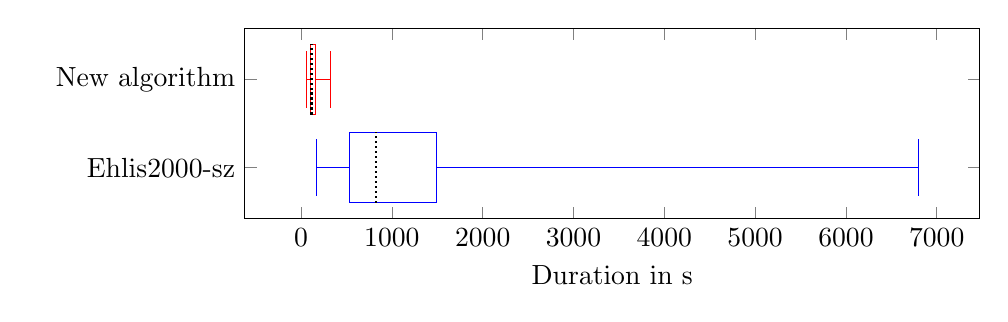
\begin{tikzpicture}
	  \begin{axis}
	    [
	    width=0.9\textwidth,
	    height=4cm,
	    ytick={1,2},
	    yticklabels={\citeauthor{Ehlis2000-sz}, New algorithm},
	    xlabel=Duration in s
	    ]
	    \addplot+[
	    boxplot prepared={
	      median=824.9113785,
	      upper quartile=1494.499004,
	      lower quartile=537.7623661,
	      upper whisker=6797.799275,
	      lower whisker=167.3832221,
	      every median/.style={densely dotted,black, thick},
	    },
	    ] coordinates {};

	    \addplot+[
	    boxplot prepared={
	      median=115.8046734,
	      upper quartile=157.223287,
	      lower quartile=108.0107692,
	      upper whisker=323.9006281,
	      lower whisker=55.58224106,
	      every median/.style={densely dotted,black, thick},
	    },
	    ] coordinates {};
	  \end{axis}
	\end{tikzpicture}
	  \vspace{-5pt}
		\caption{Average time required to execute the algorithm (150gens, 1000 population)}
		\label{fig:box_plot_algorithm_time}
	  \vspace{-10pt}
	  \end{center}
\end{figure}

\subsection{Solution size minimisation}
\label{subsec:results_size}

Finally, we were also able to obtain two datasets of the average sizes of individuals in the final population of each algorithm. These were found to not be normally distributed using a Shapiro-Wilk normality test (benchmark: W=0.926, p<0.05, our dataset: W=0.924, p<0.05), and a U-test confirmed that the difference in medians (91 nodes for our algorithm, 139.5 for the benchmark algorithm) is statistically significant (U=68, p<0.01).

\begin{wrapfigure}{r}{0.4\textwidth}
  \vspace{-50pt}
  \begin{center}
	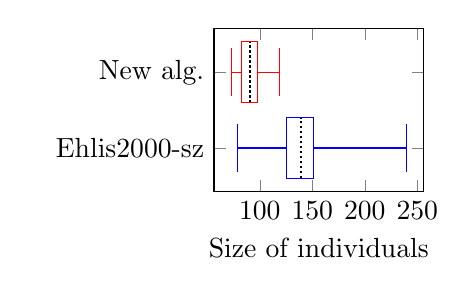
\begin{tikzpicture}
	  \begin{axis}
	    [
	    width=0.35\textwidth,
	    ytick={1,2},
	    yticklabels={\citeauthor{Ehlis2000-sz}, New alg.},
	    xlabel=Size of individuals
	    ]
	    \addplot+[
	    boxplot prepared={
	      median=139.465,
	      upper quartile=151.1725,
	      lower quartile=125.16,
	      upper whisker=239.35,
	      lower whisker=79.2,
	      every median/.style={densely dotted,black, thick},
	    },
	    ] coordinates {};

	    \addplot+[
	    boxplot prepared={
	      median=91,
	      upper quartile=98,
	      lower quartile=83,
	      upper whisker=119,
	      lower whisker=73,
	      every median/.style={densely dotted,black, thick},
	    },
	    ] coordinates {};
	  \end{axis}
	\end{tikzpicture}
	  \vspace{-5pt}
		\caption{Average number of nodes in the final generation's population}
		\label{fig:box_plot_algorithm_size}
	  \vspace{-10pt}
	  \end{center}
\end{wrapfigure}
\section{Summary \& Conclusion}
In the course of this report, we have evaluated and implemented a genetic programming algorithm proposed by \citet{Ehlis2000-sz} which aims to find a score-maximising solution to the game of Snake. This approach, which relied on a large computational power and high population size to achieve a reliable result, was discussed in \autoref{subsec:gp_snake} and analysed in \autoref{subsec:impl}; it was found to produce reliably good high-scoring snakes, in addition to a fraction of game-beating snakes, but required extremely large populations to function, and relied on mutation rather than crossover to evolve the solution. \newline

Building on this, we have developed a minimalist, non-greedy subset of operators with the aim of creating a maximal hamiltonian cycle through the map. After finding a maximally optimal set of parameters given the resources available to this project, our algorithm was evaluated in terms of the fittest individuals it could produce, the computational time required to run the algorithm, and the average size of the final population. Compared to our benchmark, our algorithm was unable to produce an equally high consistant median fitness, but could produce optimal solutions (game-beating) more consistently. It was found that, given a restricted population size and number of generations, our algorithm resulted in a near-binary best individual which would either beat the game or consistently fail on the score of 14, due to the snake boxing itself into a corner without leaving any exit path. This was caused by the strategy undertaken throughout the project, as a greedy algorithm can incrementally learn to handle each situation correctly, whereas our algorithm would either learn a complete cycle, or fail to develop the correct mutation. This could potentially be remedied by using a higher mutation rate at later stages of the evolution. \newline

Our algorithm does however produce more optimal solutions per run and per compoutational time, in addition to producing smaller solutions. These results would most likely be improved when run for a larger number of generations and a higher population, as this would increase the chance of finding a valid hamiltonian cycle throughout the game.

\subsection{Further work}

\begin{itemize}
	\item Taking a population of optimal solutions, giving them more operators and evolving a more efficient A.I. which wins the game in the smallest time possible
	\item Testing the ability to improve the reliability of the algorithm using larger populations, 
	\item Implement a meta-genetic algorithm to derive the set of operators, parameters, type of algorithm to use
\end{itemize}

\clearpage

\bibliographystyle{IEEEtranSN}
\bibliography{references}
\clearpage
\begin{appendices}
	\section{Difference in operator statistics between optimal and non-optimal solutions}
	\label{app:operator_prob}
	\begin{figure}[H]
		\centering
		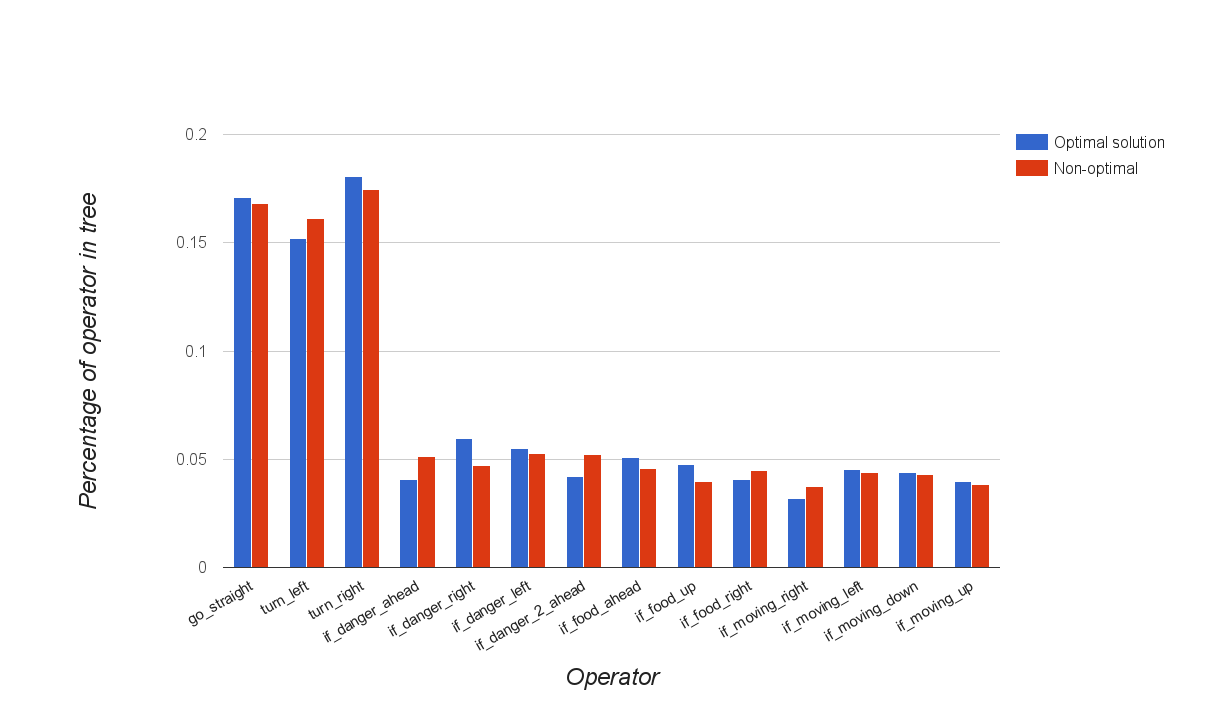
\includegraphics[width=\textwidth,keepaspectratio]{images/operator_prob.png}
		\caption{Difference in statistics of operators between optimal and non-optimal solutions}
		
	\end{figure}
	\clearpage
	\section{Parameter search graphs}
	\label{app:param_search}
	\begin{figure}[H]
		\centering
		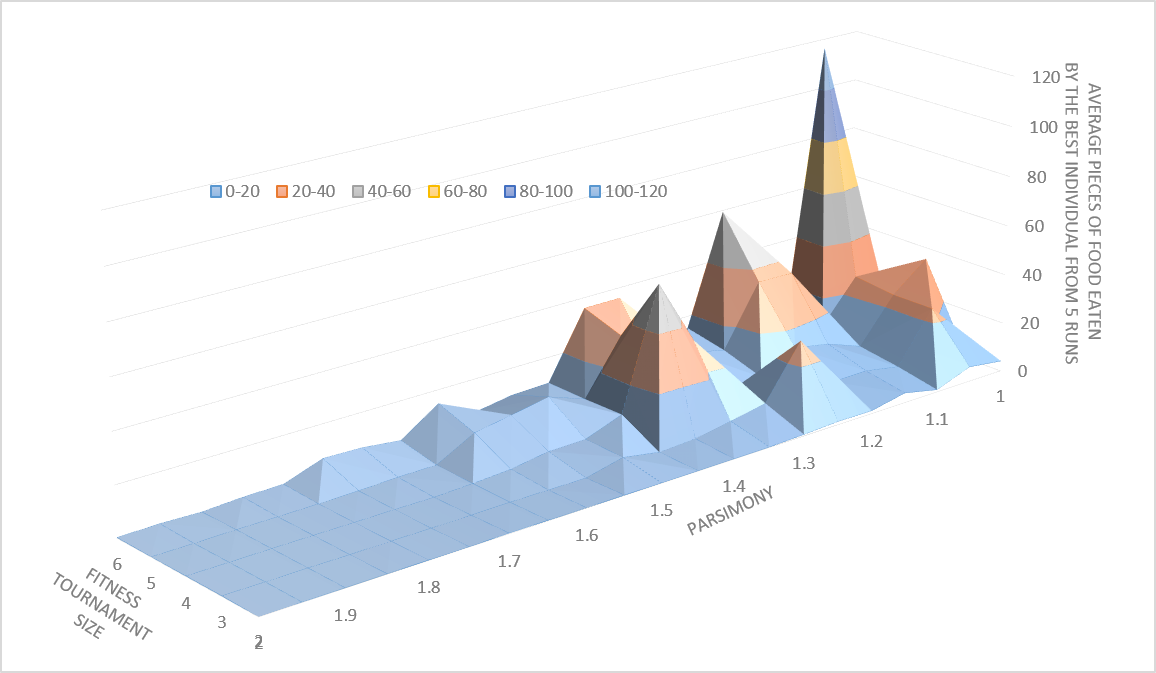
\includegraphics[width=0.7\textwidth,keepaspectratio]{images/fitness_size_parsimony.png}
		\caption{Average of 5 runs over the space of selection tournament sizes and parsimony values}
		\label{fig:fitness_parsimony}
	\end{figure}
	\begin{figure}[H]
		\centering
		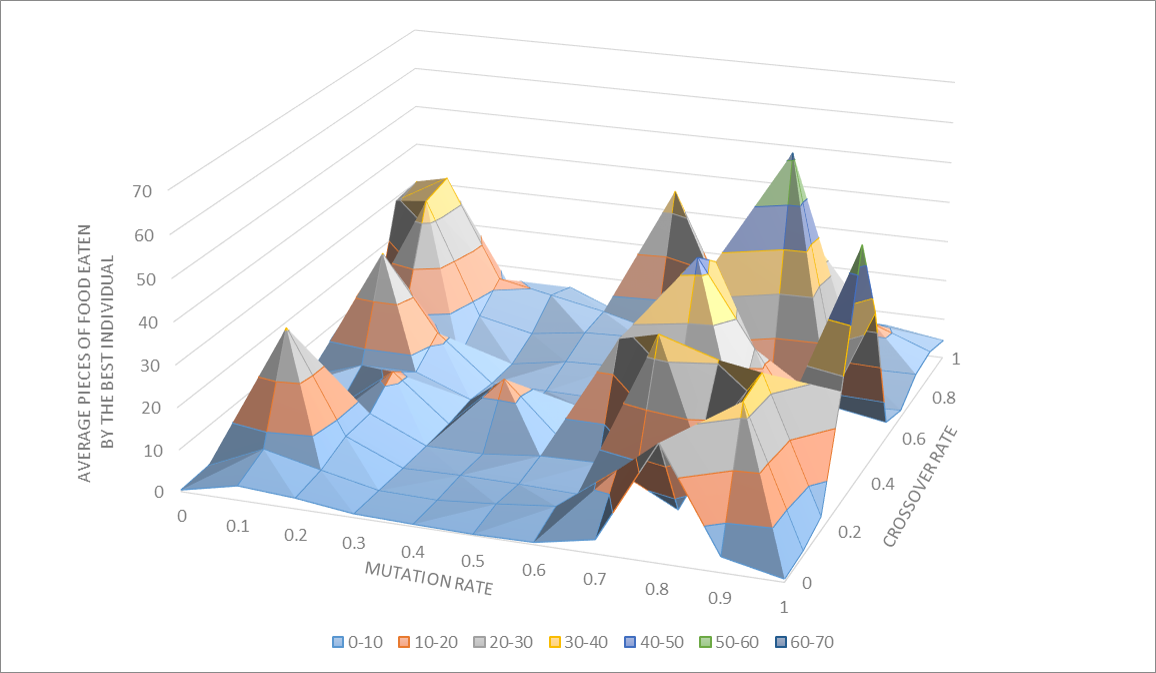
\includegraphics[width=0.7\textwidth,keepaspectratio]{images/cxpb_mutpb.png}
		\caption{Average of 5 runs over the space of mutation and crossover rates, in increments of 0.1.}
		\label{fig:mutpb_cxpb}
	\end{figure}
	\clearpage
	\section{Benchmark algorithm}\label{app:approach1}
	Based on the design document by \citet{Ehlis2000-sz}. \newline
	\lstinputlisting[language=Python]{../GP/approach1.py}
  	\clearpage	

	\section{New algorithm}\label{app:approach4}
	Based on the design document by \citet{Ehlis2000-sz}. \newline
	\lstinputlisting[language=Python]{../GP/approach4.py}
  	\clearpage	

\end{appendices}
\clearpage
\end{document}
